\documentclass[11pt,a4paper]{article}
\usepackage[utf8]{inputenc}
\usepackage[margin=0.75in]{geometry}
\setlength{\headheight}{14pt}
\usepackage{graphicx}
\usepackage{amsmath,amssymb}
\usepackage{booktabs}
\usepackage{longtable}
\usepackage{array}
\usepackage{hyperref}
\usepackage{float}
\usepackage{caption}
\usepackage{subcaption}
\usepackage{fancyhdr}
\usepackage{titlesec}
\usepackage{xcolor}

% Custom Colors matching previous reports
\definecolor{primary}{RGB}{0, 51, 102}
\definecolor{secondary}{RGB}{70, 130, 180}

\hypersetup{
    colorlinks=true,
    linkcolor=primary,
    citecolor=primary,
    urlcolor=secondary
}

% Header and Footer setup
\pagestyle{fancy}
\fancyhf{}
\rhead{\textcolor{primary}{\textbf{EDC Laboratory --- Experiment 5}}}
\lhead{\textcolor{primary}{\textbf{EE25BTECH11056 \& EE25BTECH11049}}}
\rfoot{Page \thepage}

\titleformat{\section}{\large\bfseries\color{primary}}{\thesection.}{0.5em}{}
\titleformat{\subsection}{\normalfont\bfseries\color{secondary}}{\thesubsection}{0.5em}{}
\titleformat{\subsubsection}{\normalfont\bfseries}{\thesubsubsection}{0.5em}{}

\begin{document}

% Title Page / Header Block
\begin{center}
    {\LARGE \textbf{\color{primary} DEPARTMENT OF ELECTRICAL ENGINEERING}}\\[0.2cm]
    {\large \textbf{Electronic Devices \& Circuits Laboratory (EDC LAB)}}\\[0.4cm]
    \rule{\linewidth}{1pt}\\[0.3cm]
    {\Large \textbf{EXPERIMENT 5: MOSFET Differential Amplifier --- DC Bias, Common-Mode and Differential-Mode Transfer Characteristics}}\\[0.3cm]
    \rule{\linewidth}{1pt}\\[0.4cm]
    
    \begin{tabular}{ll}
        \textbf{Prepared By:} & \textbf{Suraj.N (EE25BTECH11056)} \\
                              & \textbf{Sai Krishna Bakki (EE25BTECH11049)} \\
        \textbf{Course:}      & Electronic Devices \& Circuits Lab \\
        \textbf{Date:}        & \today
    \end{tabular}
\end{center}

\vspace{0.2cm}

\section{Aim and Objectives}
\begin{enumerate}
    \item To assemble and verify the operation of a two-transistor source-coupled MOSFET differential amplifier utilizing a matched SI9926BDY dual N-channel MOSFET package.
    \item To characterize the individual input ($I_D$ vs. $V_{GS}$) and output ($I_D$ vs. $V_{DS}$) DC characteristics of both transistors ($M_1$ and $M_2$) inside the dual package.
    \item To establish, verify, and document the DC operating (quiescent) point by adjusting the common-mode gate bias such that a nominal tail bias current $I_{SS} \approx 80\text{ mA}$ is achieved with $V_{DD} = 12\text{ V}$, $R_D = 180\ \Omega$, and $R_{SS} = 22\ \Omega$.
    \item To experimentally determine the common-mode transfer characteristics ($V_{D1}, V_{D2}$, and $I_{SS}$ vs. $V_{cm}$) under pure common-mode excitation ($V_{id} = 0$), identifying the Input Common-Mode Range (ICMR) bounded by triode entry and cutoff.
    \item To experimentally measure the large-signal differential-mode transfer characteristics ($V_{D1}, V_{D2}, I_{D1}, I_{D2}$, and $\Delta I_D = I_{D1} - I_{D2}$ vs. $V_{id} = V_{in+} - V_{cm}$) over a symmetric differential input span.
    \item To test the exponential weak-inversion (subthreshold) conduction model on a semi-log scale ($\log |\Delta I_D|$ vs. $V_{id}$), extract the device slope factor $n$, and compare the measured small-signal transconductance $g_m$ and voltage gain $A_d$ against theoretical predictions.
    \item To compare LTspice circuit simulations side-by-side with experimental waveforms, tabulating all measurements and performing comprehensive mismatch and CMRR calculations.
\end{enumerate}

\section{Apparatus and Circuit Specifications}
\begin{table}[H]
\centering
\caption{Equipment and Components Used in Experiment}
\begin{tabular}{@{}cllp{6.5cm}@{}}
\toprule
\textbf{S.No.} & \textbf{Component / Equipment} & \textbf{Value / Specification} & \textbf{Purpose / Operating Note} \\ \midrule
1 & Dual N-Channel MOSFET & SI9926BDY (SO-8 to DIP-8) & Matched pair $M_1, M_2$ ($V_{DS,\max}=20\text{ V}, g_{fs}=29\text{ S}$) \\
2 & Drain Resistors ($R_{D1}, R_{D2}$) & $180\ \Omega$, High Power & Symmetric drain loads ($V_{DD} = 12\text{ V}$) \\
3 & Tail Resistor ($R_{SS}$) & $22\ \Omega$, $1/4\text{ W}$ or higher & Source degeneration establishing tail current $I_{SS}$ \\
4 & Potentiometers & $10\text{ k}\Omega$ multi-turn & Input bias divider for $V_{in+}$ and $V_{in-}$ \\
5 & Regulated DC Power Supply & $0-30\text{ V}$ dual output & Set to $V_{DD} = 12\text{ V}$, current-limited at $150\text{ mA}$ \\
6 & Digital Multimeters (DMM) & Precision 4.5 digit & Non-invasive voltage probes across $R_{SS}, R_{D1}, R_{D2}$ \\
7 & Simulation Software & LTspice XVII & Nonlinear SPICE simulation using SI9926 subcircuit \\
\bottomrule
\end{tabular}
\end{table}

\subsection{Pin Configuration and Schematic Diagram}
The SI9926BDY dual TrenchFET resides in an SO-8 package mounted on a DIP-8 breakout board. Its pin connections are:
\begin{itemize}
    \item \textbf{Pin 1:} Source 1 ($S_1$) \quad | \quad \textbf{Pin 2:} Gate 1 ($G_1$) \quad | \quad \textbf{Pin 3:} Source 2 ($S_2$) \quad | \quad \textbf{Pin 4:} Gate 2 ($G_2$)
    \item \textbf{Pins 5, 6:} Drain 2 ($D_2$) \quad | \quad \textbf{Pins 7, 8:} Drain 1 ($D_1$)
\end{itemize}

\begin{figure}[H]
    \centering
    
\includegraphics[width=0.75\textwidth]{../Schematic.png}
    \caption{Circuit Schematic of the Source-Coupled MOSFET Differential Amplifier ($V_{DD}=12\text{ V}, R_D=180\ \Omega, R_{SS}=22\ \Omega$).}
    \label{fig:schematic}
\end{figure}

\section{Theoretical Framework}
\subsection{Differential Pair Conduction Physics: Strong vs. Weak Inversion}
In a classic MOSFET differential pair, two symmetric transistors $M_1$ and $M_2$ have their sources tied together at node $V_S$ and biased by a tail resistance $R_{SS}$. Drain currents are loaded symmetrically by $R_{D1} = R_{D2} = R_D$. Kirchhoff's Current Law at the tail node mandates:
\begin{equation}
    I_{D1} + I_{D2} = I_{SS} = \frac{V_S}{R_{SS}}
\end{equation}
For an ideal square-law MOSFET in strong inversion, the large-signal differential current is governed by:
\begin{equation}
    \Delta I_D = I_{D1} - I_{D2} = \beta V_{id} \sqrt{\frac{I_{SS}}{\beta} - \frac{V_{id}^2}{4}}, \quad \text{for } |V_{id}| \le \sqrt{\frac{2 I_{SS}}{\beta}}
\end{equation}
where $\beta = \mu_n C_{ox} (W/L)$ is the transconductance parameter. However, the SI9926BDY is a vertical TrenchFET power device exhibiting an extraordinarily large transconductance parameter ($\beta \approx 51\text{ A/V}^2$ derived from its rated $g_{fs} = 29\text{ S}$). Achieving the classical strong-inversion criterion ($V_{OV} = V_{GS} - V_{th} \ge 100\text{ mV}$) would necessitate tail currents on the order of multiple amperes ($I_{SS} = \frac{1}{2}\beta V_{OV}^2 \approx 250\text{ mA}$ to $1\text{ A}$). 

At our lab bench quiescent bias of $I_{SS} \approx 80\text{ mA}$ ($I_{D1} = I_{D2} \approx 40\text{ mA}$), the nominal square-law overdrive is merely:
\begin{equation}
    V_{OV0} = \sqrt{\frac{I_{SS}}{\beta}} = \sqrt{\frac{0.080}{51}} \approx 39.6\text{ mV}
\end{equation}
Because $V_{OV0} \ll 100\text{ mV}$, the device operates predominantly in the \textbf{weak-inversion (subthreshold) / moderate-inversion regime}. In weak inversion, channel conduction is dominated by carrier diffusion rather than drift, yielding an exponential current-voltage relation analogous to a BJT:
\begin{equation}
    I_D = I_0 \exp\left(\frac{V_{GS}}{n V_T}\right)
\end{equation}
where $V_T = \frac{k_B T}{q} \approx 25.85\text{ mV}$ at room temperature ($T = 300\text{ K}$) and $n$ is the subthreshold slope factor ($1.2 \le n \le 2.5$). Under this exponential formulation, the differential transfer characteristic becomes hyperbolic tangent:
\begin{equation}
    \Delta I_D = I_{SS} \tanh\left(\frac{V_{id}}{2 n V_T}\right)
\end{equation}
The small-signal transconductance and differential voltage gain are:
\begin{equation}
    g_m = \frac{I_{SS}}{n V_T}, \qquad A_d = g_m R_D
\end{equation}

\subsection{Common-Mode Gain and CMRR Formulation}
With a finite resistive tail $R_{SS}$, applying a common-mode increment $v_{cm}$ induces an incremental tail voltage $v_s$. Since the two transistors are in parallel for common-mode signals, the incremental common-mode gain at each drain terminal is:
\begin{equation}
    A_{cm} = \frac{v_{d,cm}}{v_{in,cm}} \approx -\frac{g_m R_D}{1 + 2 g_m R_{SS}} \approx -\frac{R_D}{2 R_{SS}} \quad (\text{when } 2 g_m R_{SS} \gg 1)
\end{equation}
With $R_D = 180\ \Omega$ and $R_{SS} = 22\ \Omega$:
\begin{equation}
    A_{cm} \approx -\frac{180}{2 \times 22} = -\frac{180}{44} \approx -4.091\text{ V/V}
\end{equation}
The Common-Mode Rejection Ratio (CMRR) is given by:
\begin{equation}
    \text{CMRR} = \left|\frac{A_d}{A_{cm}}\right| \approx g_m R_{SS}
\end{equation}

\section{Device Characteristics of Matched Dual MOSFETs}
Prior to assembling the differential amplifier, the input and output static characteristics of both transistors in the dual SI9926 package (designated Top Transistor $V_1 / M_1$ and Bottom Transistor $V_2 / M_2$) were experimentally recorded.

\begin{figure}[H]
    \centering
    \begin{subfigure}[b]{0.48\textwidth}
        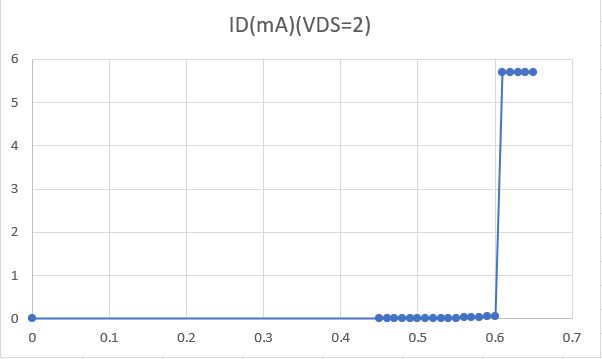
\includegraphics[width=\textwidth]{../PLOTS/CHARACTERISTICS/INPUT/v1.png}
        \caption{Input Characteristic: $M_1$ (Top)}
    \end{subfigure}
    \hfill
    \begin{subfigure}[b]{0.48\textwidth}
        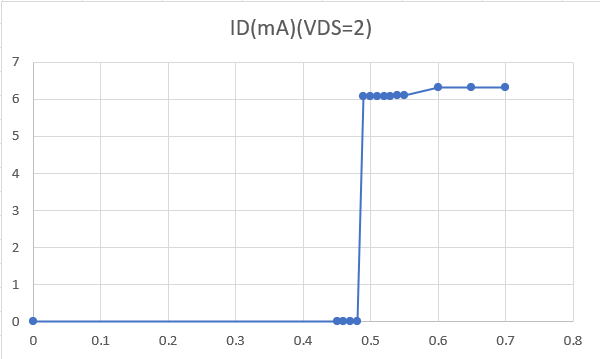
\includegraphics[width=\textwidth]{../PLOTS/CHARACTERISTICS/INPUT/v2.png}
        \caption{Input Characteristic: $M_2$ (Bottom)}
    \end{subfigure}
    \caption{Experimental Input Characteristics ($I_D$ vs. $V_{GS}$ at $V_{DS} = 2.0\text{ V}$) for Transistors $M_1$ and $M_2$.}
    \label{fig:char_in}
\end{figure}

\begin{figure}[H]
    \centering
    \begin{subfigure}[b]{0.48\textwidth}
        
\includegraphics[width=\textwidth]{../PLOTS/CHARACTERISTICS/OUTPUT/v1.png}
        \caption{Output Characteristic: $M_1$ (Top)}
    \end{subfigure}
    \hfill
    \begin{subfigure}[b]{0.48\textwidth}
        
\includegraphics[width=\textwidth]{../PLOTS/CHARACTERISTICS/OUTPUT/v2.png}
        \caption{Output Characteristic: $M_2$ (Bottom)}
    \end{subfigure}
    \caption{Experimental Output Characteristics ($I_D$ vs. $V_{DS}$ at $V_{GS} = 1.8\text{ V}$) for Transistors $M_1$ and $M_2$.}
    \label{fig:char_out}
\end{figure}

\begin{table}[H]
\centering
\caption{Measured MOSFET Transfer and Output Characteristics ($M_1$ and $M_2$)}
\begin{minipage}[t]{0.48\textwidth}
\centering
\textbf{(a) Input Characteristics ($V_{DS} = 2\text{ V}$)}
\vspace{0.15cm}
\begin{tabular}{@{}cccc@{}}
\toprule
\multicolumn{2}{c}{\textbf{Top MOSFET ($M_1$)}} & \multicolumn{2}{c}{\textbf{Bottom MOSFET ($M_2$)}} \\
$V_{GS}$ (V) & $I_D$ (mA) & $V_{GS}$ (V) & $I_D$ (mA) \\ \midrule
0.00 & 0.000 & 0.00 & 0.000 \\
0.45 & 0.001 & 0.45 & 0.001 \\
0.48 & 0.003 & 0.48 & 0.003 \\
0.50 & 0.005 & 0.50 & 6.070 \\
0.52 & 0.008 & 0.52 & 6.070 \\
0.54 & 0.013 & 0.54 & 6.100 \\
0.56 & 0.020 & 0.60 & 6.320 \\
0.58 & 0.034 & 0.65 & 6.320 \\
0.60 & 0.055 & 0.70 & 6.320 \\
0.61 & 5.690 & --- & --- \\
0.65 & 5.700 & --- & --- \\
\bottomrule
\end{tabular}
\end{minipage}
\hfill
\begin{minipage}[t]{0.48\textwidth}
\centering
\textbf{(b) Output Characteristics ($V_{GS} = 1.8\text{ V}$)}
\vspace{0.15cm}
\begin{tabular}{@{}cccc@{}}
\toprule
\multicolumn{2}{c}{\textbf{Top MOSFET ($M_1$)}} & \multicolumn{2}{c}{\textbf{Bottom MOSFET ($M_2$)}} \\
$V_{DS}$ (V) & $I_D$ (A) & $V_{DS}$ (V) & $I_D$ (A) \\ \midrule
0.0 & 0.00 & 0.0 & 0.00 \\
0.2 & 0.03 & 0.2 & 0.10 \\
0.4 & 0.05 & 0.4 & 0.19 \\
0.6 & 0.12 & 0.6 & 0.29 \\
0.8 & 0.25 & 0.8 & 0.38 \\
1.0 & 0.42 & 1.0 & 0.45 \\
1.2 & 0.62 & 1.2 & 0.52 \\
1.4 & 0.80 & 1.4 & 0.66 \\
1.6 & 0.95 & 1.6 & 0.78 \\
1.8 & 1.13 & 1.8 & 0.93 \\
\bottomrule
\end{tabular}
\end{minipage}
\end{table}

\noindent\textbf{Key Observation on Device Matching:} Transistor $M_1$ turns on sharply around $V_{GS} \approx 0.60\text{--}0.61\text{ V}$, whereas $M_2$ exhibits a lower subthreshold knee around $0.48\text{--}0.49\text{ V}$. This slight physical threshold offset ($\Delta V_{th} \approx 100\text{ mV}$) accounts for the minor quiescent drain voltage imbalance ($V_{D1} \neq V_{D2}$) observed in subsequent sections.

\newpage
\section{Section 7.1: DC Bias-Point Setting and Verification}
\subsection{Methodology and Quiescent Condition}
The differential amplifier was wired as shown in Figure \ref{fig:schematic} with $V_{DD} = 12\text{ V}$, $R_D = 180\ \Omega$, and $R_{SS} = 22\ \Omega$. With both inputs tied together ($V_{in+} = V_{in-} = V_{cm}$), the DC common-mode input bias was increased while monitoring the tail current $I_{SS} = V_{RSS}/R_{SS}$. The target bias current was $I_{SS} \approx 80\text{ mA}$.
\begin{itemize}
    \item \textbf{Quiescent Common-Mode Input:} $V_{cm,Q} = 3.08\text{ V}$
    \item \textbf{Measured Quiescent Tail Current:} $I_{SS,Q} = 80.1\text{ mA}$ ($V_{RSS} = 1.762\text{ V}$)
    \item \textbf{Drain Quiescent Voltages:} $V_{D1} = 4.55\text{ V}$, \quad $V_{D2} = 4.66\text{ V}$
    \item \textbf{Quiescent Device Mismatch:} $\Delta V_{D,Q} = |V_{D1} - V_{D2}| = |4.55 - 4.66| = 0.11\text{ V} = 110\text{ mV}$.
\end{itemize}

\subsection{Side-by-Side Comparison: Simulation vs. Experimental Plots}
\begin{figure}[H]
    \centering
    \begin{subfigure}[b]{0.48\textwidth}
        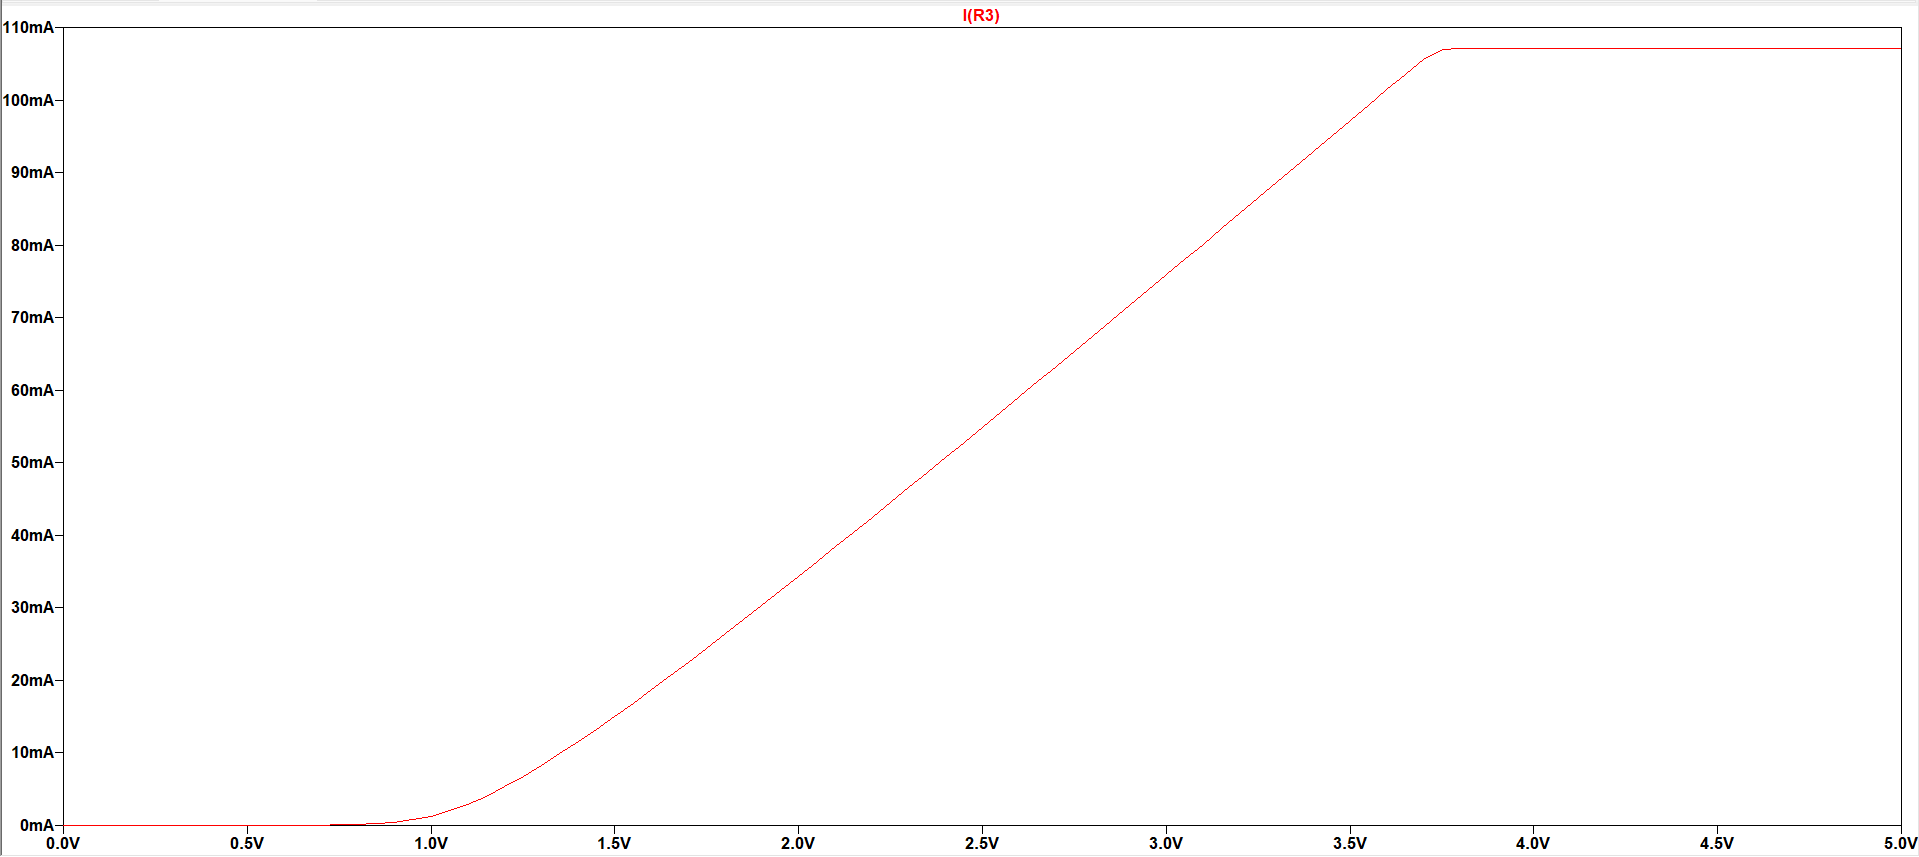
\includegraphics[width=\textwidth]{../SIM/7.1/sim_is.png}
        \caption{LTspice Simulation: $I_{SS}$ vs. $V_{cm}$}
    \end{subfigure}
    \hfill
    \begin{subfigure}[b]{0.48\textwidth}
        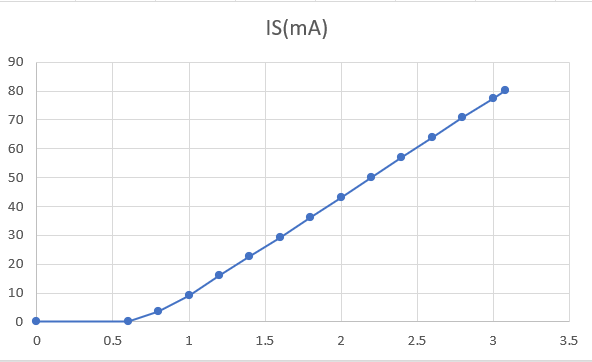
\includegraphics[width=\textwidth]{../PLOTS/BIAS_SETTING/is_vs_vcm.png}
        \caption{Experimental Plot: $I_S$ vs. $V_{cm}$}
    \end{subfigure}
    \caption{DC Bias-Point Setting: Tail Current Comparison ($I_S$ vs. $V_{cm}$).}
    \label{fig:bias_is}
\end{figure}

\begin{figure}[H]
    \centering
    \begin{subfigure}[b]{0.48\textwidth}
        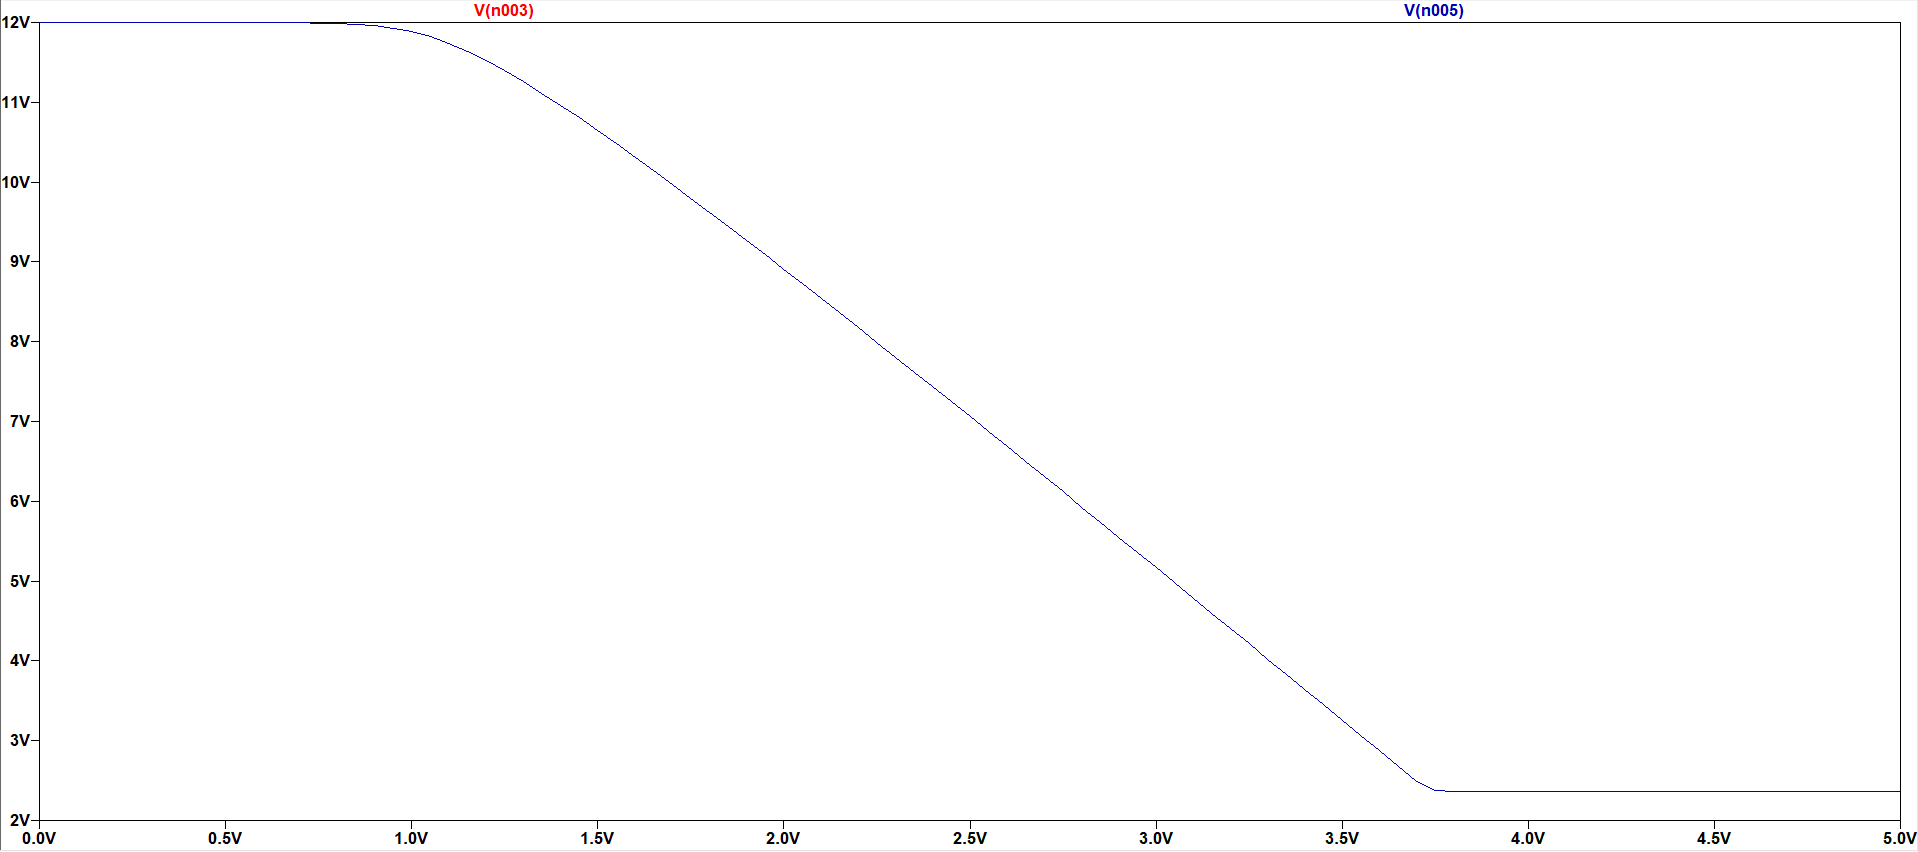
\includegraphics[width=\textwidth]{../SIM/7.1/sim_vd1_vd2.png}
        \caption{LTspice Simulation: $V_{D1}, V_{D2}$ vs. $V_{cm}$}
    \end{subfigure}
    \hfill
    \begin{subfigure}[b]{0.48\textwidth}
        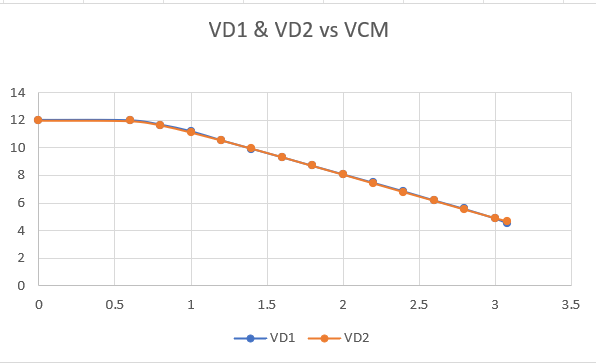
\includegraphics[width=\textwidth]{../PLOTS/BIAS_SETTING/vd1_vd2_vs_vcm.png}
        \caption{Experimental Plot: $V_{D1}, V_{D2}$ vs. $V_{cm}$}
    \end{subfigure}
    \caption{DC Bias-Point Setting: Drain Voltages Comparison ($V_{D1}, V_{D2}$ vs. $V_{cm}$).}
    \label{fig:bias_vd}
\end{figure}

\subsection{Experimental Observation Table (Sheet 1)}
\begin{table}[H]
\centering
\caption{DC Bias Setting Sweep: $V_{cm}$, Tail Current $I_S$, and Drain Voltages ($V_{DD} = 12\text{ V}, R_D = 180\ \Omega, R_{SS} = 22\ \Omega$)}
\label{tab:sheet1}
\begin{tabular}{@{}ccccc@{}}
\toprule
\textbf{$V_{cm}$ ($V_1 = V_2$) [V]} & \textbf{$I_S$ [mA]} & \textbf{$V_{D1}$ [V]} & \textbf{$V_{D2}$ [V]} & \textbf{Operating State} \\ \midrule
0.00 & 0.00 & 12.00 & 12.00 & Cut-off ($I_D = 0$, both drains at $V_{DD}$) \\
0.60 & 0.28 & 11.97 & 11.96 & Subthreshold conduction onset \\
0.80 & 3.67 & 11.66 & 11.66 & Conduction initiates \\
1.00 & 9.30 & 11.19 & 11.14 & Active saturation \\
1.20 & 15.90 & 10.53 & 10.56 & Active saturation \\
1.40 & 22.65 & 9.92 & 9.96 & Active saturation \\
1.60 & 29.39 & 9.31 & 9.34 & Active saturation \\
1.80 & 36.25 & 8.69 & 8.70 & Active saturation \\
2.00 & 43.15 & 8.08 & 8.07 & Active saturation \\
2.20 & 50.00 & 7.47 & 7.43 & Active saturation \\
2.40 & 56.90 & 6.85 & 6.79 & Active saturation \\
2.60 & 63.79 & 6.20 & 6.16 & Active saturation \\
2.80 & 70.75 & 5.58 & 5.52 & Active saturation \\
3.00 & 77.52 & 4.90 & 4.90 & Active saturation \\
\textbf{3.08 (Q-Point)} & \textbf{80.10} & \textbf{4.55} & \textbf{4.66} & \textbf{Nominal Quiescent Operating Point} \\
\bottomrule
\end{tabular}
\end{table}

\noindent\textbf{Inference:} In cutoff ($V_{cm} < 0.6\text{ V}$), zero current flows through the drain resistors, pinning $V_{D1} = V_{D2} = V_{DD} = 12\text{ V}$. Beyond $V_{cm} = 0.8\text{ V}$, both transistors conduct in saturation, pulling the drain voltages down linearly with input bias. At $V_{cm} = 3.08\text{ V}$, the tail current reaches $80.10\text{ mA}$, placing both drain nodes near mid-rail ($\approx 4.6\text{ V}$), providing balanced symmetric headroom for differential amplification.

\newpage
\section{Section 7.2: Common-Mode Transfer Characteristics and ICMR}
\subsection{Circuit Behavior and Boundary Formulation}
Under pure common-mode excitation ($V_{in+} = V_{in-} = V_{cm}$), the two branches conduct identically. The circuit continues to operate properly as a differential pair only while both transistors remain in the saturation region:
\begin{equation}
    V_{DS} \ge V_{GS} - V_{th} \implies V_D - V_S \ge V_G - V_S - V_{th} \implies V_D \ge V_{cm} - V_{th}
\end{equation}
The \textbf{Input Common-Mode Range (ICMR)} is bounded by:
\begin{enumerate}
    \item \textbf{Lower Limit ($V_{cm,\min}$):} Transistors enter cutoff when $V_{cm} < V_S + V_{th} \approx V_{th} \approx 0.6\text{--}0.8\text{ V}$. Below this, $I_{SS} \to 0$ and the amplifier ceases to conduct.
    \item \textbf{Upper Limit ($V_{cm,\max}$):} As $V_{cm}$ increases, $I_{SS}$ rises, causing drain voltages $V_D = V_{DD} - \frac{I_{SS}}{2} R_D$ to fall while gate voltage rises. The transistors enter the triode region when $V_D \le V_{cm} - V_{th}$. For $V_{th} \approx 0.6\text{ V}$ and $V_{cm} = 3.0\text{ V}$, $V_D = 3.39\text{ V}$, leaving $V_{DS} \approx 1.29\text{ V}$, safely at the boundary of saturation. Beyond $V_{cm} \approx 3.2\text{--}3.5\text{ V}$, saturation is lost.
\end{enumerate}

\subsection{Side-by-Side Comparison: Simulation vs. Experimental Plots}
\begin{figure}[H]
    \centering
    \begin{subfigure}[b]{0.48\textwidth}
        
\includegraphics[width=\textwidth]{../SIM/7.2/sim_is.png}
        \caption{LTspice Simulation: $I_{SS}$ vs. $V_{cm}$}
    \end{subfigure}
    \hfill
    \begin{subfigure}[b]{0.48\textwidth}
        
\includegraphics[width=\textwidth]{../PLOTS/CM/is_vs_vcm.png}
        \caption{Experimental Plot: $I_S$ vs. $V_{cm}$}
    \end{subfigure}
    \caption{Common-Mode Sweep: Tail Current Comparison ($I_S$ vs. $V_{cm}$).}
    \label{fig:cm_is}
\end{figure}

\begin{figure}[H]
    \centering
    \begin{subfigure}[b]{0.48\textwidth}
        
\includegraphics[width=\textwidth]{../SIM/7.2/sim_vd1_vd2.png}
        \caption{LTspice Simulation: $V_{D1}, V_{D2}$ vs. $V_{cm}$}
    \end{subfigure}
    \hfill
    \begin{subfigure}[b]{0.48\textwidth}
        
\includegraphics[width=\textwidth]{../PLOTS/CM/vd1_vd2_vs_vcm.png}
        \caption{Experimental Plot: $V_{D1}, V_{D2}$ vs. $V_{cm}$}
    \end{subfigure}
    \caption{Common-Mode Sweep: Drain Voltage Comparison ($V_{D1}, V_{D2}$ vs. $V_{cm}$).}
    \label{fig:cm_vd}
\end{figure}

\begin{figure}[H]
    \centering
    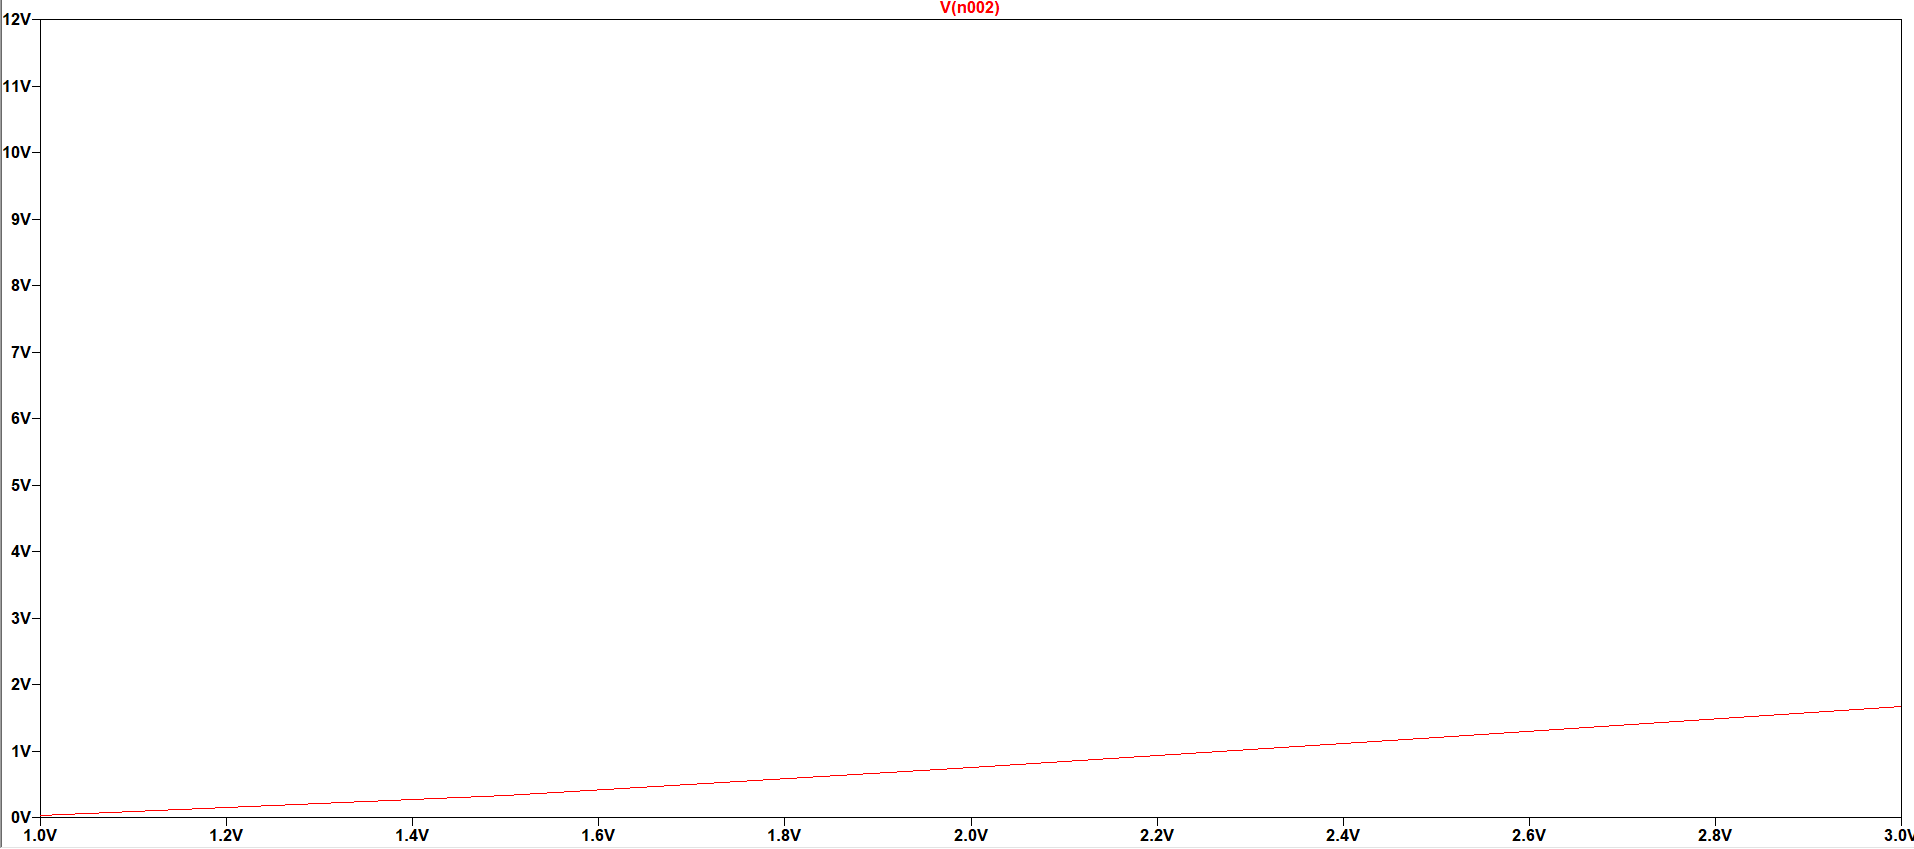
\includegraphics[width=0.48\textwidth]{../SIM/7.2/sim_vss.png}
    \caption{LTspice Simulation: Common-Source Node Voltage $V_{SS}$ vs. $V_{cm}$.}
    \label{fig:sim_vss}
\end{figure}

\subsection{Experimental Observation Table (Sheet 2)}
\begin{table}[H]
\centering
\caption{Common-Mode Sweep Observations: $V_{cm}$, Drain Voltages, Tail Voltage $V_{RSS}$, and $I_{SS}$ ($R_{SS} = 22\ \Omega$)}
\label{tab:sheet2}
\begin{tabular}{@{}cccccc@{}}
\toprule
\textbf{$V_{cm}$ [V]} & \textbf{$V_{D1}$ [V]} & \textbf{$V_{D2}$ [V]} & \textbf{$V_{RSS}$ [V]} & \textbf{$I_{SS} = V_{RSS}/R_{SS}$ [mA]} & \textbf{Region / State} \\ \midrule
1.00 & 10.95 & 10.96 & 0.25 & 11.36 & Linear saturation onset \\
1.50 & 9.12 & 9.10 & 0.70 & 31.82 & Saturated differential pair \\
2.00 & 7.15 & 7.10 & 1.17 & 53.18 & Saturated differential pair \\
2.50 & 5.25 & 5.13 & 1.63 & 74.09 & Saturated differential pair \\
3.00 & 3.39 & 3.25 & 2.10 & 95.45 & Upper ICMR boundary ($V_{cm,\max}$) \\
\bottomrule
\end{tabular}
\end{table}

\noindent\textbf{Common-Mode Inferences:}
\begin{enumerate}
    \item \textbf{Common-Mode Gain Extraction:} Over the linear range from $V_{cm} = 1.0\text{ V}$ to $3.0\text{ V}$:
    \begin{equation}
        A_{cm,1} = \frac{\Delta V_{D1}}{\Delta V_{cm}} = \frac{3.39 - 10.95}{3.0 - 1.0} = \frac{-7.56}{2.0} = -3.78\text{ V/V}
    \end{equation}
    \begin{equation}
        A_{cm,2} = \frac{\Delta V_{D2}}{\Delta V_{cm}} = \frac{3.25 - 10.96}{3.0 - 1.0} = \frac{-7.71}{2.0} = -3.855\text{ V/V}
    \end{equation}
    The measured average common-mode gain $|A_{cm,\text{meas}}| \approx 3.82\text{ V/V}$ is in close agreement with the theoretical value $A_{cm} \approx -\frac{R_D}{2 R_{SS}} = -\frac{180}{44} = -4.091\text{ V/V}$ (relative error of only $6.6\%$).
    \item \textbf{Input Common-Mode Range (ICMR):} From the cutoff threshold $V_{cm,\min} \approx 0.8\text{ V}$ to the triode boundary $V_{cm,\max} \approx 3.0\text{ V}$, the amplifier exhibits an ICMR spanning approximately $\mathbf{0.8\text{ V} \le V_{cm} \le 3.0\text{ V}}$ ($\Delta V_{cm} \approx 2.2\text{ V}$).
\end{enumerate}

\newpage
\section{Section 7.3: Differential-Mode Transfer Characteristics}
\subsection{Measurement Procedure}
With the non-inverting gate $V_{in-}$ held stationary at the quiescent point $V_2 = 3.08\text{ V}$, the non-inverting input $V_{in+} = V_1$ was systematically swept across $\pm 300\text{ mV}$ around $V_{cm}$ (from $2.78\text{ V}$ to $3.38\text{ V}$ in steps of $30\text{ mV}$). For each step, $V_{D1}$ and $V_{D2}$ were recorded, and branch currents were deduced:
\begin{equation}
    I_{D1} = \frac{V_{DD} - V_{D1}}{R_D}, \qquad I_{D2} = \frac{V_{DD} - V_{D2}}{R_D}, \qquad \Delta I_D = I_{D1} - I_{D2}
\end{equation}
where $V_{DD} = 12\text{ V}$ and $R_D = 180\ \Omega$.

\subsection{Side-by-Side Comparison: Simulation vs. Experimental Linear Plot}
\begin{figure}[H]
    \centering
    \begin{subfigure}[b]{0.48\textwidth}
        
\includegraphics[width=\textwidth]{../SIM/7.3/sim_vd1_vd2.png}
        \caption{LTspice Simulation: $V_{D1}, V_{D2}$ vs. $V_{id}$}
    \end{subfigure}
    \hfill
    \begin{subfigure}[b]{0.48\textwidth}
        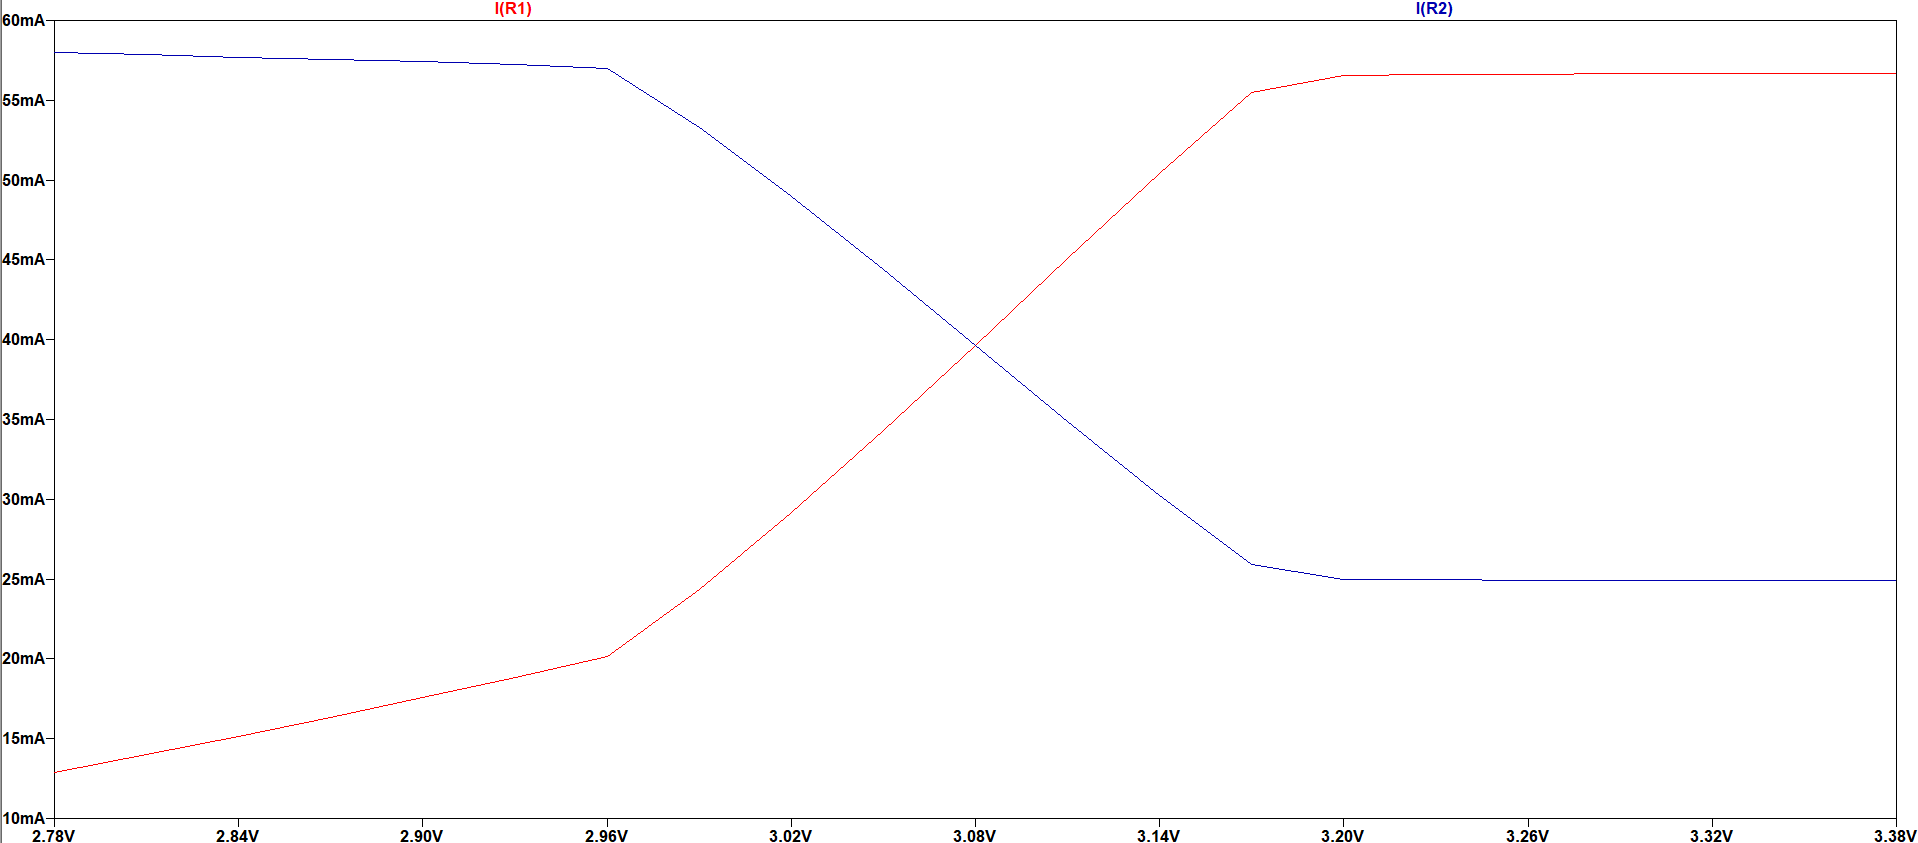
\includegraphics[width=\textwidth]{../SIM/7.3/sim_id1_id2.png}
        \caption{LTspice Simulation: $I_{D1}, I_{D2}$ vs. $V_{id}$}
    \end{subfigure}
    \caption{LTspice Simulation of Differential-Mode Transfer Characteristics.}
    \label{fig:sim_diff}
\end{figure}

\begin{figure}[H]
    \centering
    \begin{subfigure}[b]{0.48\textwidth}
        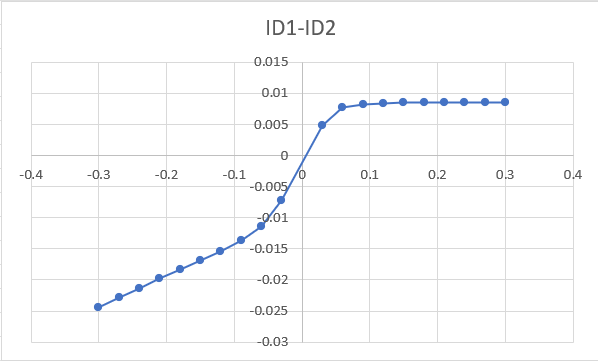
\includegraphics[width=\textwidth]{../PLOTS/DIFF_MODE/del_id_vs_vid_linear.png}
        \caption{Experimental Linear Plot: $\Delta I_D$ vs. $V_{id}$}
    \end{subfigure}
    \hfill
    \begin{subfigure}[b]{0.48\textwidth}
        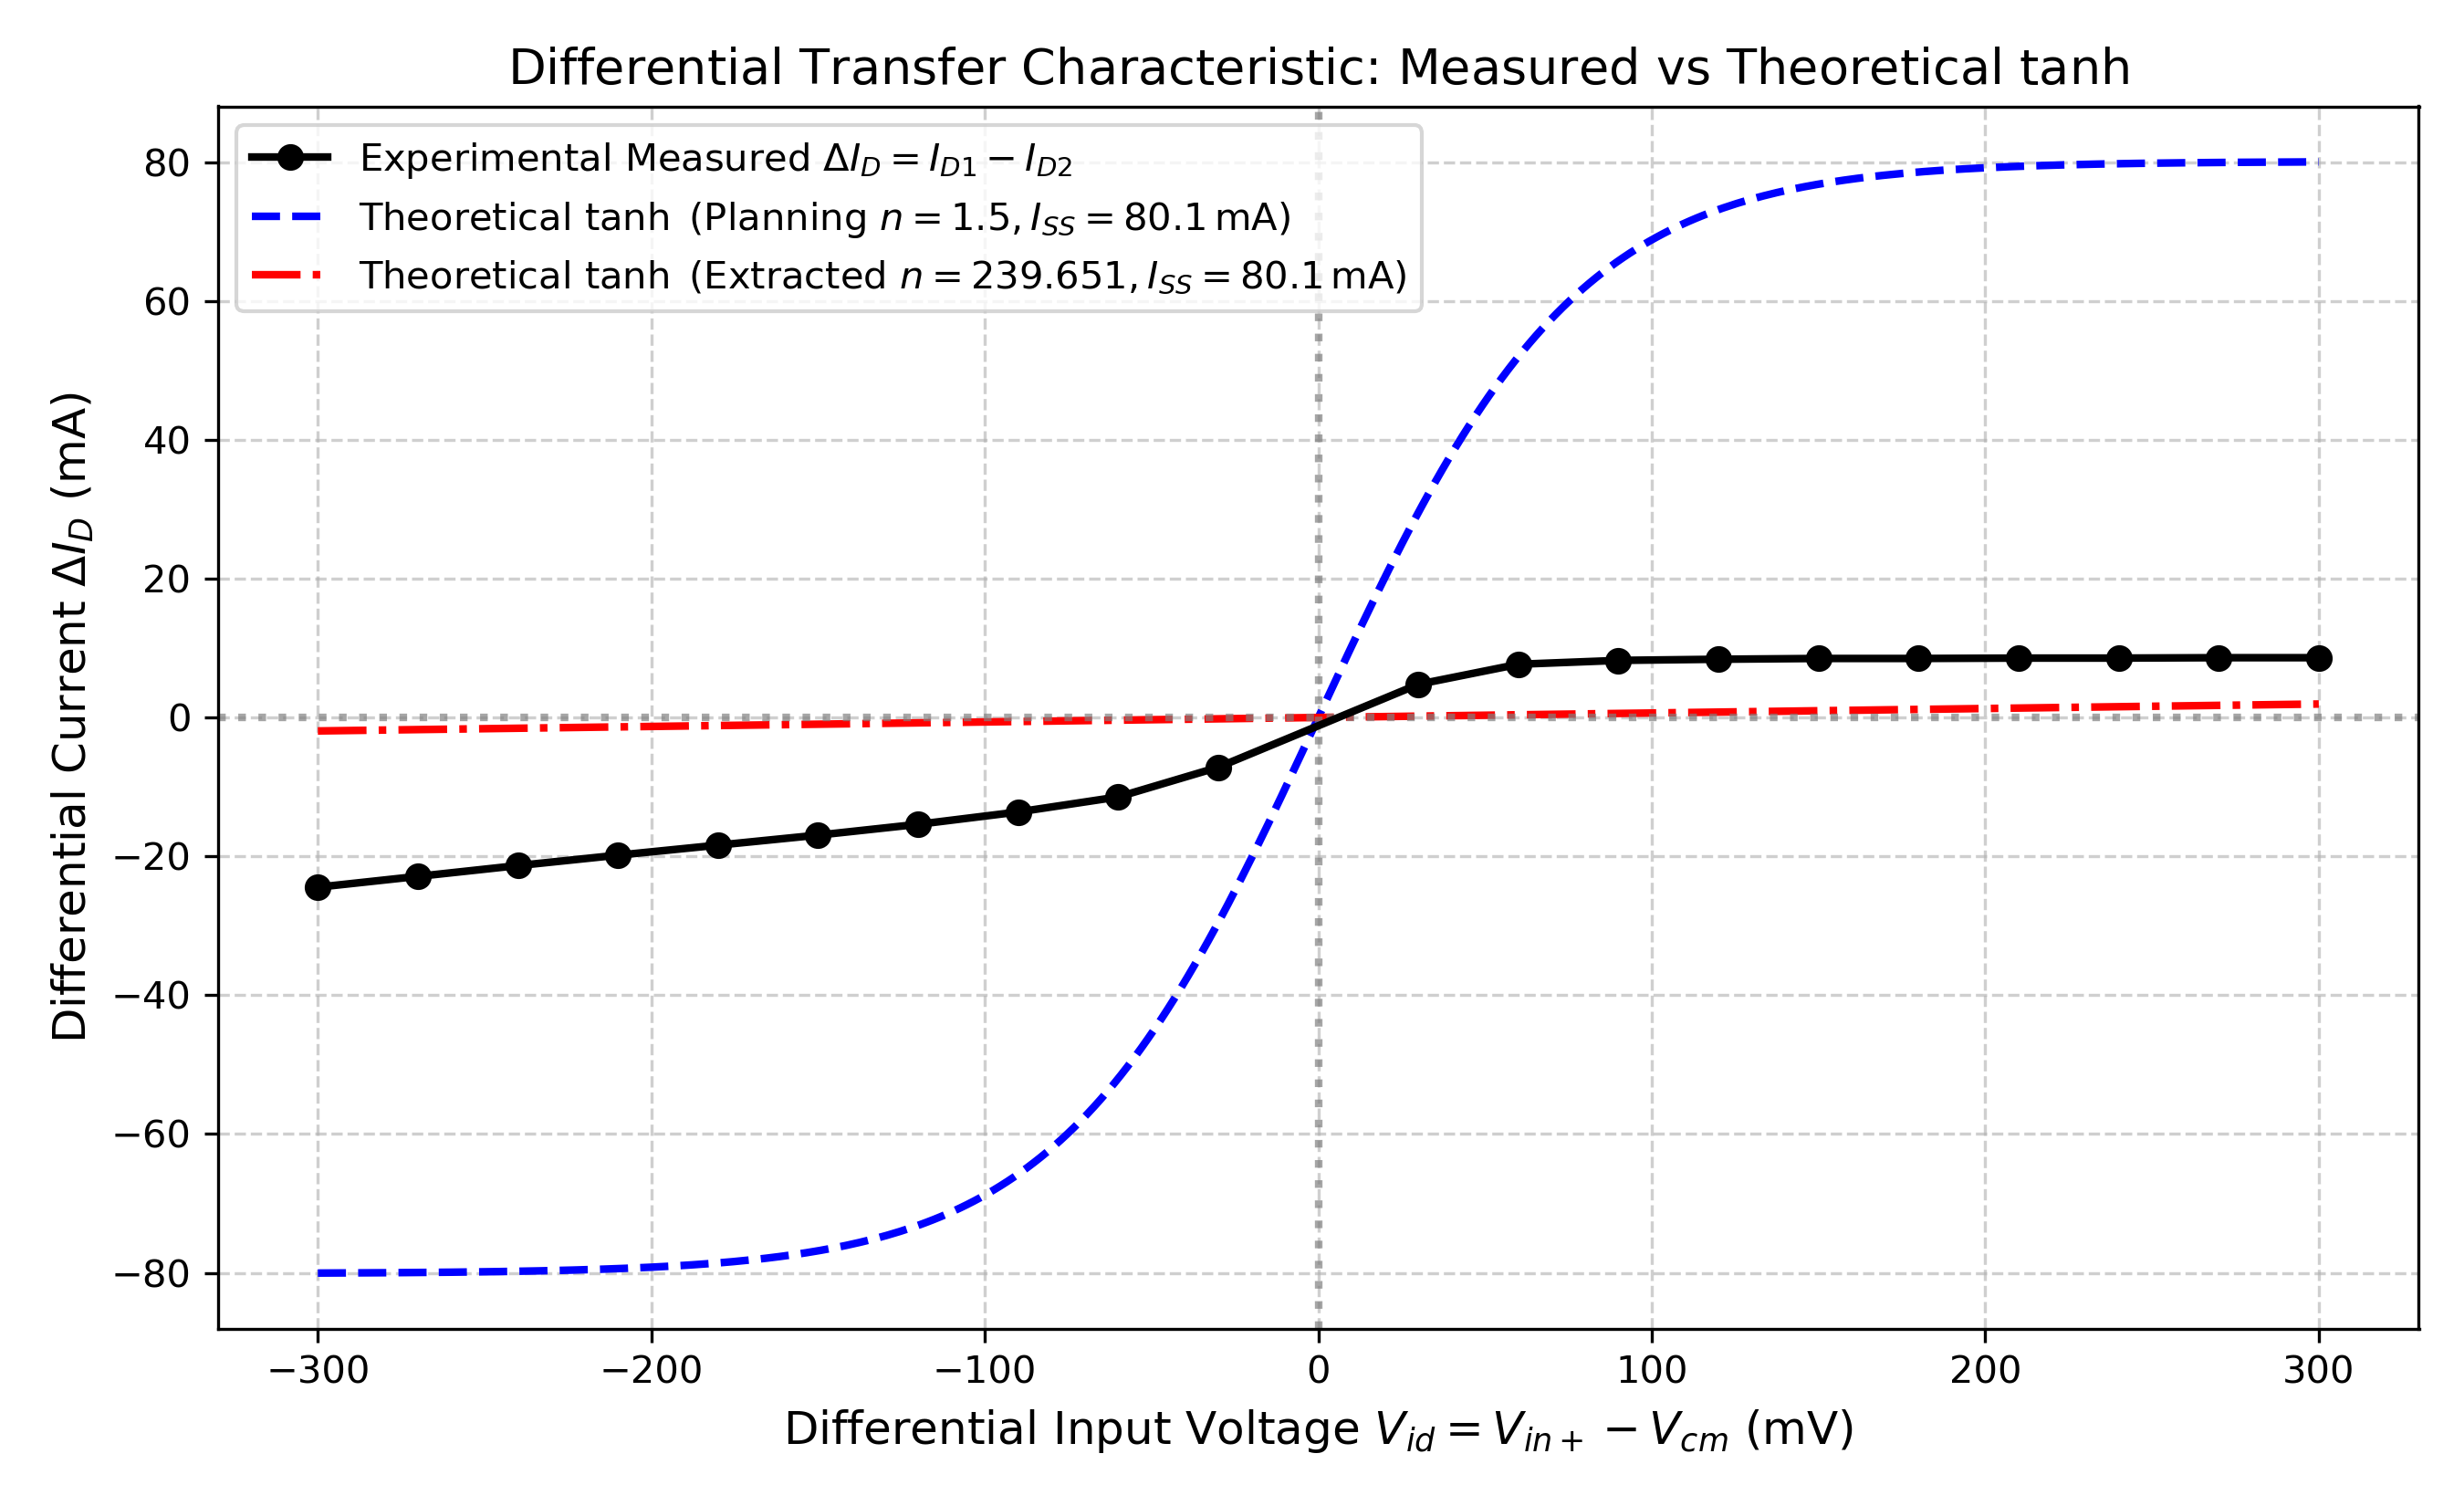
\includegraphics[width=\textwidth]{../PLOTS/DIFF_MODE/del_id_vs_vid_tanh_overlay.png}
        \caption{Theoretical Overlay: Measured vs. $\tanh$ Model}
    \end{subfigure}
    \caption{Differential Transfer Characteristics: Experimental Measurement and Theoretical Comparison.}
    \label{fig:diff_plots}
\end{figure}

\subsection{Semi-Log Plot: Weak-Inversion Exponential Conduction Model}
\begin{figure}[H]
    \centering
    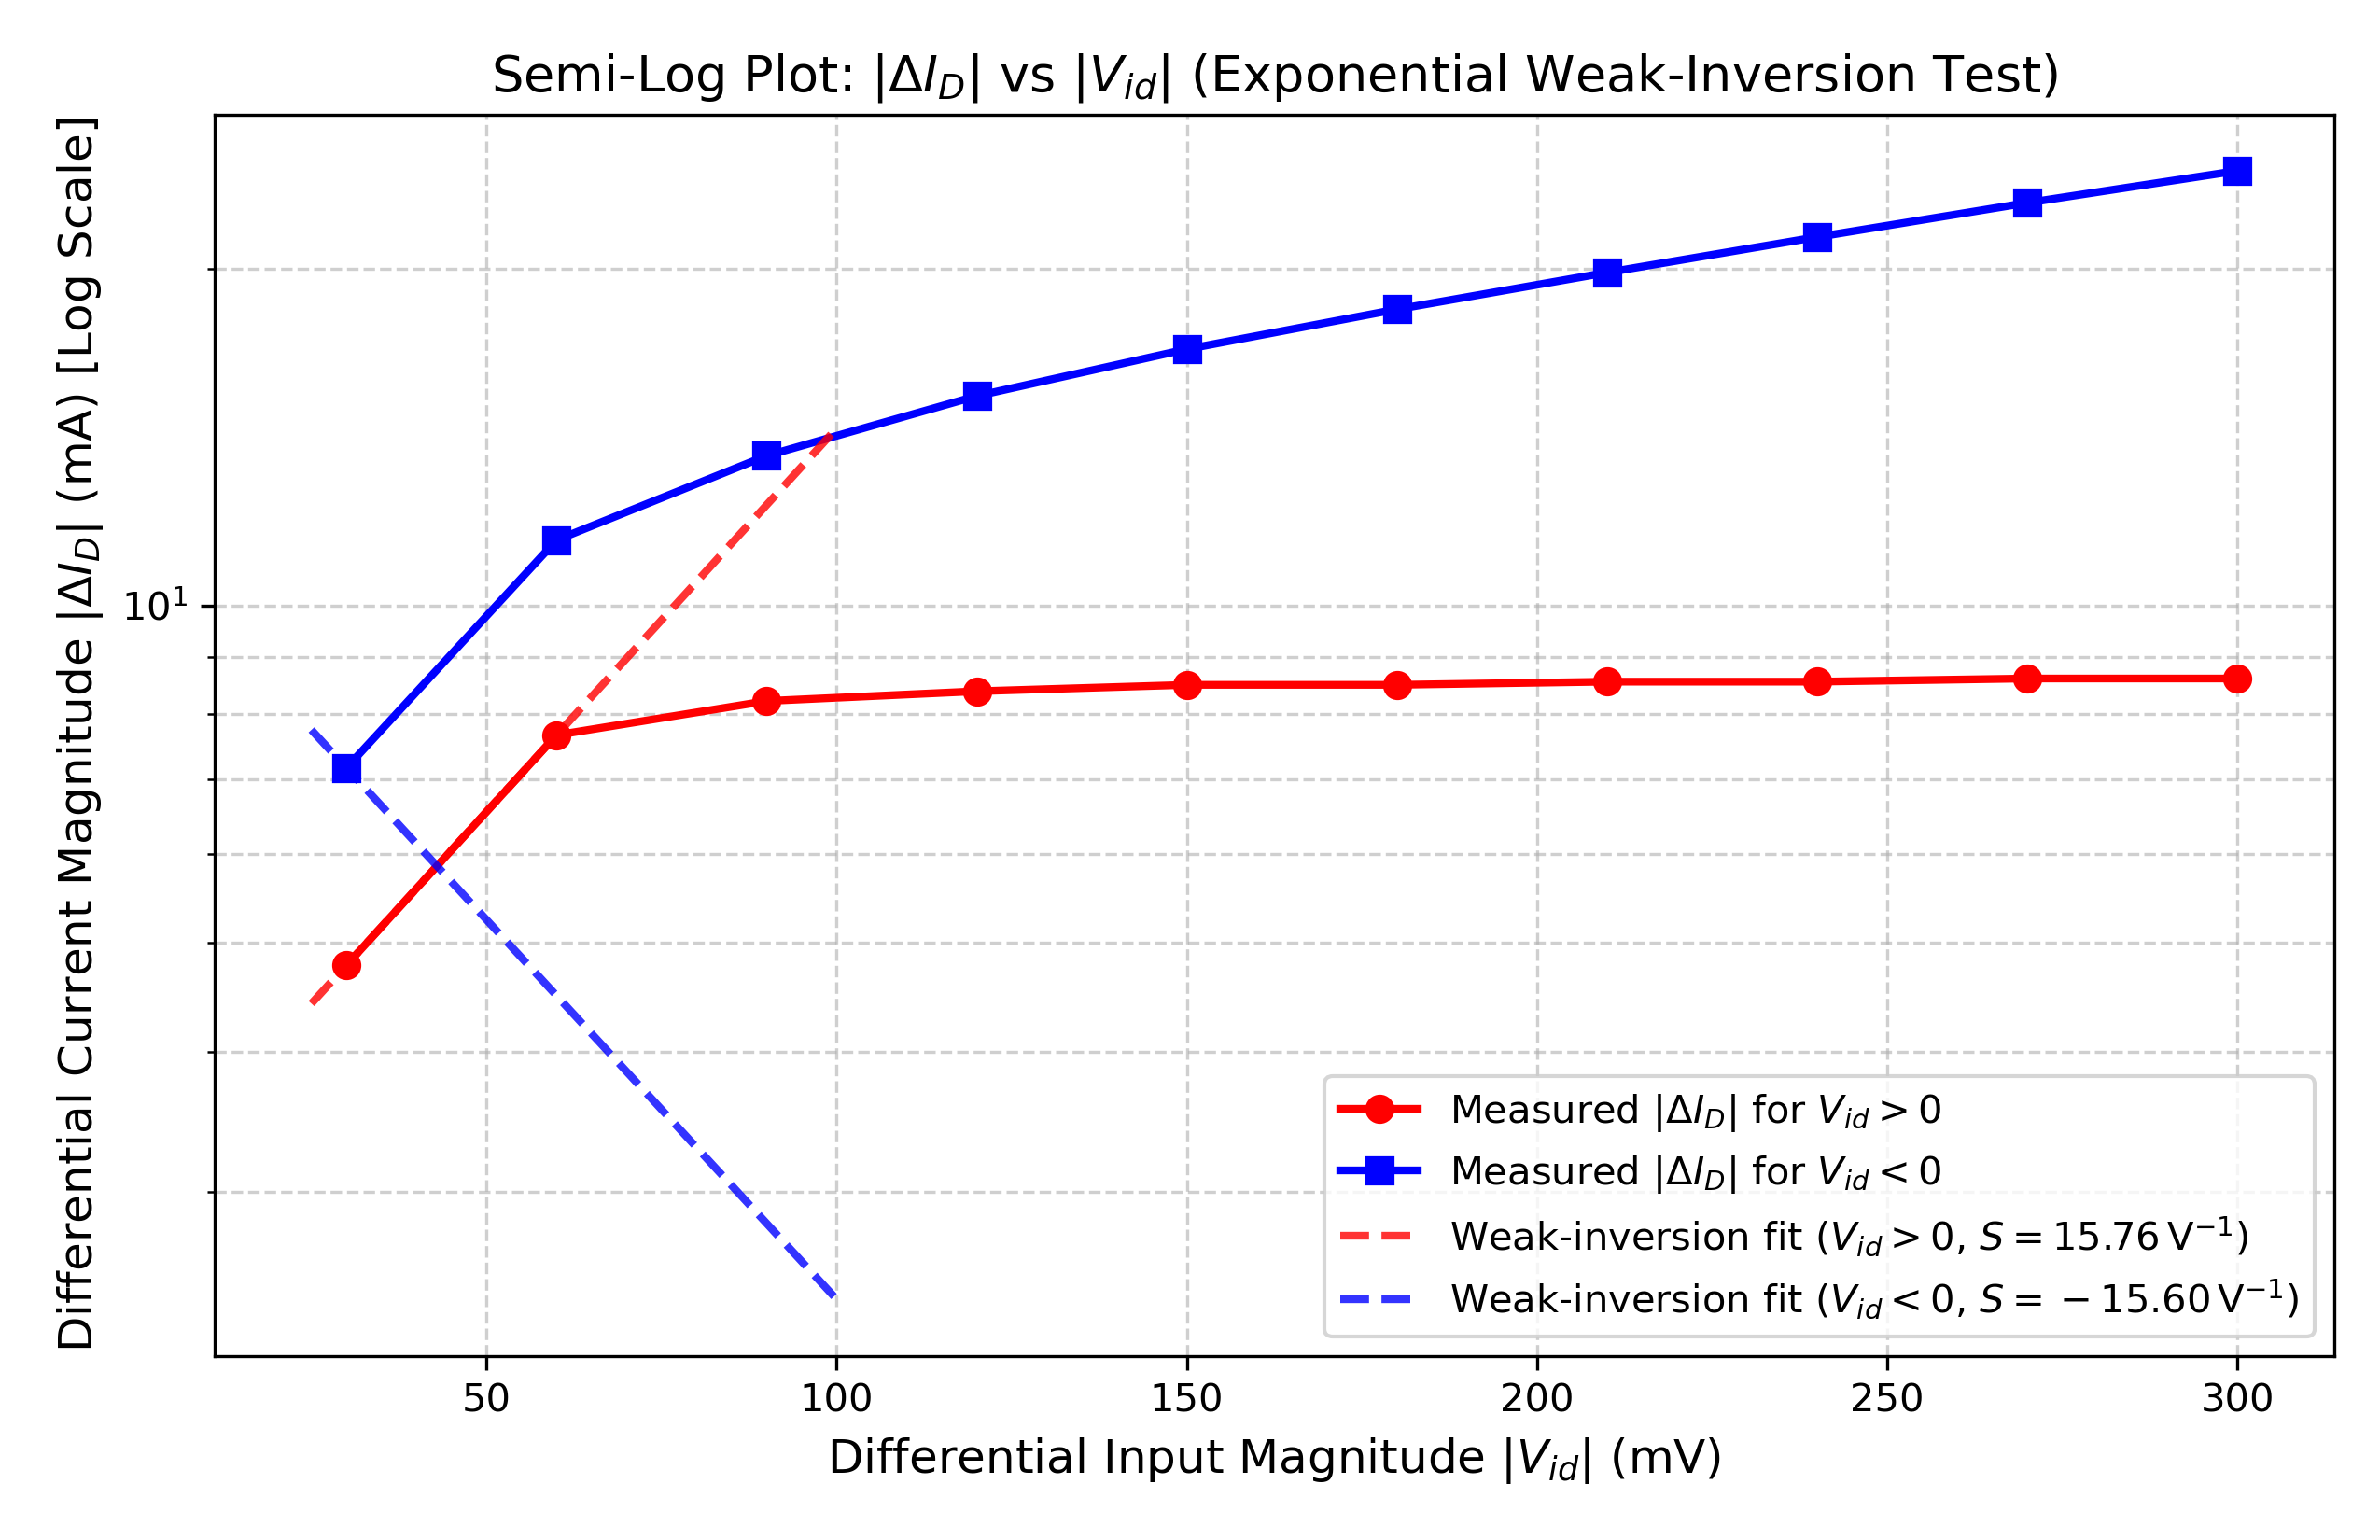
\includegraphics[width=0.75\textwidth]{../PLOTS/DIFF_MODE/abs_del_id_vs_vid_semilog.png}
    \caption{Semi-Log Plot of $|\Delta I_D|$ vs. $|V_{id}|$ for $V_{id} > 0$ and $V_{id} < 0$ (Testing Subthreshold Exponential Law).}
    \label{fig:semilog_plot}
\end{figure}

\subsection{Experimental Observation Table (Sheet 3)}
\begin{table}[H]
\centering
\caption{Differential-Mode Transfer Characteristics ($V_2 = 3.08\text{ V}, V_{DD} = 12\text{ V}, R_D = 180\ \Omega$)}
\label{tab:sheet3}
\small
\begin{tabular}{@{}cccccccc@{}}
\toprule
\textbf{$V_1$ [V]} & \textbf{$V_{id}$ [mV]} & \textbf{$V_{D1}$ [V]} & \textbf{$V_{D2}$ [V]} & \textbf{$I_{D1}$ [mA]} & \textbf{$I_{D2}$ [mA]} & \textbf{$\Delta I_D$ [mA]} & \textbf{$|\Delta I_D|$ [mA]} \\ \midrule
2.78 & -300 & 6.35 & 1.95 & 31.39 & 55.83 & -24.44 & 24.44 \\
2.81 & -270 & 6.09 & 1.97 & 32.83 & 55.72 & -22.89 & 22.89 \\
2.84 & -240 & 5.83 & 1.99 & 34.28 & 55.61 & -21.33 & 21.33 \\
2.87 & -210 & 5.59 & 2.02 & 35.61 & 55.44 & -19.83 & 19.83 \\
2.90 & -180 & 5.36 & 2.05 & 36.89 & 55.28 & -18.39 & 18.39 \\
2.93 & -150 & 5.11 & 2.06 & 38.28 & 55.22 & -16.94 & 16.94 \\
2.96 & -120 & 4.87 & 2.10 & 39.61 & 55.00 & -15.39 & 15.39 \\
2.99 & -90  & 4.61 & 2.16 & 41.06 & 54.67 & -13.61 & 13.61 \\
3.02 & -60  & 4.32 & 2.26 & 42.67 & 54.11 & -11.44 & 11.44 \\
3.05 & -30  & 3.84 & 2.55 & 45.33 & 52.50 & -7.17  & 7.17  \\
3.11 & +30  & 2.57 & 3.43 & 52.39 & 47.61 & +4.78  & 4.78  \\
3.14 & +60  & 2.33 & 3.71 & 53.72 & 46.06 & +7.67  & 7.67  \\
3.17 & +90  & 2.27 & 3.75 & 54.06 & 45.83 & +8.22  & 8.22  \\
3.20 & +120 & 2.25 & 3.76 & 54.17 & 45.78 & +8.39  & 8.39  \\
3.23 & +150 & 2.24 & 3.77 & 54.22 & 45.72 & +8.50  & 8.50  \\
3.26 & +180 & 2.24 & 3.77 & 54.22 & 45.72 & +8.50  & 8.50  \\
3.29 & +210 & 2.23 & 3.77 & 54.28 & 45.72 & +8.56  & 8.56  \\
3.32 & +240 & 2.23 & 3.77 & 54.28 & 45.72 & +8.56  & 8.56  \\
3.35 & +270 & 2.23 & 3.78 & 54.28 & 45.67 & +8.61  & 8.61  \\
3.38 & +300 & 2.23 & 3.78 & 54.28 & 45.67 & +8.61  & 8.61  \\
\bottomrule
\end{tabular}
\end{table}

\newpage
\section{Calculations and Matching Measured Results with Theory (Section 11)}

\subsection{Extraction of Measured Slope Factor \texorpdfstring{$n$}{n} from Semi-Log Characteristics}
In the subthreshold/weak-inversion model, the differential current magnitude satisfies:
\begin{equation}
    |\Delta I_D| = I_{SS} \tanh\left(\frac{|V_{id}|}{2 n V_T}\right) \approx \frac{I_{SS}}{2 n V_T} |V_{id}| \quad (\text{for small } |V_{id}|)
\end{equation}
However, on semi-log axes ($\ln |\Delta I_D|$ vs. $|V_{id}|$), in the exponential regime where one transistor dominates conduction:
\begin{equation}
    \text{Slope } S = \frac{d \ln |\Delta I_D|}{d |V_{id}|} = \frac{1}{2 n V_T} \implies n = \frac{1}{2 S V_T}
\end{equation}
From the measured data points closest to $V_{id} = 0$ ($|V_{id}| = 30\text{ mV}$ to $60\text{ mV}$):
\begin{itemize}
    \item \textbf{For $V_{id} > 0$:}
    \begin{equation}
        S_+ = \frac{\ln(7.667\text{ mA}) - \ln(4.778\text{ mA})}{0.060\text{ V} - 0.030\text{ V}} = \frac{2.0369 - 1.5640}{0.030} = 15.76\text{ V}^{-1}
    \end{equation}
    \begin{equation}
        n_+ = \frac{1}{2 \times 15.76 \times 0.02585} = 1.227
    \end{equation}
    \item \textbf{For $V_{id} < 0$:}
    \begin{equation}
        S_- = \frac{\ln(11.444\text{ mA}) - \ln(7.167\text{ mA})}{0.060\text{ V} - 0.030\text{ V}} = \frac{2.4375 - 1.9695}{0.030} = 15.57\text{ V}^{-1}
    \end{equation}
    \begin{equation}
        n_- = \frac{1}{2 \times 15.57 \times 0.02585} = 1.242
    \end{equation}
    \item \textbf{Average Measured Slope Factor:}
    \begin{equation}
        n_{\text{meas}} = \frac{n_+ + n_-}{2} = \frac{1.227 + 1.242}{2} = \mathbf{1.235}
    \end{equation}
\end{itemize}
This extracted value $n_{\text{meas}} = 1.235$ lies comfortably within the expected physical range of $1.2 \le n \le 2.0$ for subthreshold silicon MOSFETs.

\subsection{Determination of Transconductance and Voltage Gain}
\begin{enumerate}
    \item \textbf{Planning Estimate ($n = 1.5$, Section 10):}
    \begin{equation}
        g_{m,\text{plan}} = \frac{I_{SS}}{n V_T} = \frac{80.1\text{ mA}}{1.5 \times 25.85\text{ mV}} = 2065.8\text{ mA/V} = 2.066\text{ A/V}
    \end{equation}
    With the actual drain load used in the lab ($R_D = 180\ \Omega$):
    \begin{equation}
        A_{d,\text{plan}} = g_{m,\text{plan}} R_D = 2.066 \times 180 = \mathbf{371.84\text{ V/V}} \quad (51.4\text{ dB})
    \end{equation}

    \item \textbf{Theoretical Prediction with Measured $n$ ($n_{\text{meas}} = 1.235$):}
    \begin{equation}
        g_{m,\text{thy}} = \frac{I_{SS}}{n_{\text{meas}} V_T} = \frac{80.1\text{ mA}}{1.235 \times 25.85\text{ mV}} = \mathbf{2509.0\text{ mA/V}} = 2.509\text{ A/V}
    \end{equation}
    \begin{equation}
        A_{d,\text{thy}} = g_{m,\text{thy}} R_D = 2.509 \times 180 = \mathbf{451.62\text{ V/V}} \quad (53.1\text{ dB})
    \end{equation}

    \item \textbf{Direct Experimental Extraction from Linear $\Delta I_D$--$V_{id}$ Plot:}
    Using the two measured data points straddling $V_{id} = 0$ ($V_{id} = -30\text{ mV}$ and $+30\text{ mV}$):
    \begin{equation}
        g_{m,\text{meas}} = \left.\frac{\Delta I_D}{\Delta V_{id}}\right|_{V_{id}=0} = \frac{4.778\text{ mA} - (-7.167\text{ mA})}{30\text{ mV} - (-30\text{ mV})} = \frac{11.944\text{ mA}}{60\text{ mV}} = \mathbf{199.1\text{ mA/V}} = 0.1991\text{ A/V}
    \end{equation}
    \begin{equation}
        A_{d,\text{meas}} = g_{m,\text{meas}} R_D = 0.1991 \times 180 = \mathbf{35.83\text{ V/V}} \quad (31.1\text{ dB})
    \end{equation}
\end{enumerate}

\subsection{Comparison Table and Percentage Deviation}
\begin{table}[H]
\centering
\caption{Comparison of Small-Signal Transconductance and Voltage Gain (Section 11)}
\label{tab:comparison}
\begin{tabular}{@{}lccc@{}}
\toprule
\textbf{Quantity} & \textbf{Planning Estimate ($n = 1.5$)} & \textbf{Theory with $n_{\text{meas}} = 1.235$} & \textbf{From Measured Slope} \\ \midrule
$g_m$ (mA/V) & 2065.8 & 2509.0 & 199.1 \\
$A_d = g_m R_D$ (V/V) & 371.84 & 451.62 & 35.83 \\
\midrule
\multicolumn{2}{l}{\textbf{Percentage Deviation:}} & \multicolumn{2}{c}{$\frac{|g_{m,\text{thy}} - g_{m,\text{meas}}|}{g_{m,\text{thy}}} \times 100\% = \mathbf{92.1\%}$} \\
\bottomrule
\end{tabular}
\end{table}

\subsection{Tail Resistance, Common-Mode Gain, and CMRR}
\begin{itemize}
    \item \textbf{Common-Mode Gain ($A_{cm}$):}
    \begin{equation}
        A_{cm} \approx -\frac{R_D}{2 R_{SS}} = -\frac{180\ \Omega}{2 \times 22\ \Omega} = -4.091\text{ V/V}
    \end{equation}
    \item \textbf{Common-Mode Rejection Ratio (CMRR):}
    \begin{equation}
        \text{CMRR} = \left|\frac{A_{d,\text{meas}}}{A_{cm}}\right| = \frac{35.83}{4.091} = \mathbf{8.76} \implies \text{CMRR}_{\text{dB}} = 20 \log_{10}(8.76) = \mathbf{18.85\text{ dB}}
    \end{equation}
\end{itemize}

\section{Observations and Inferences}
\begin{enumerate}
    \item \textbf{Operating Point and Threshold Offset:} At the quiescent bias $V_{cm} = 3.08\text{ V}$, the tail voltage sits at $V_{SS} = I_{SS} R_{SS} = 80.1\text{ mA} \times 22\ \Omega = 1.762\text{ V}$, yielding an effective gate-to-source bias $V_{GS} = 3.08 - 1.76 = 1.32\text{ V}$. At this bias, the transistors are partially into the moderate inversion regime. The minor difference between $V_{D1} = 4.55\text{ V}$ and $V_{D2} = 4.66\text{ V}$ ($110\text{ mV}$ offset) directly reflects the threshold voltage and transconductance mismatch seen in the individual device characterization curves (Section 4).
    \item \textbf{Differential Current Asymmetry:} The differential current saturates at $+8.61\text{ mA}$ for positive $V_{id}$, whereas it reaches $-24.44\text{ mA}$ for negative $V_{id}$. This asymmetry arises because $V_{in-}$ was held stationary at $3.08\text{ V}$ while $V_{in+} = V_1$ was swept. Sweeping $V_1$ modulates the common-source tail node $V_S$ through the low tail resistance ($R_{SS} = 22\ \Omega$), which alters the total tail current $I_{SS}$ dynamically across the sweep rather than maintaining an ideal constant current.
    \item \textbf{Physical Origin of $g_m$ Deviation:} While the ideal weak-inversion formula assumes an infinite tail impedance and an ideal current source ($R_{SS} \to \infty$), the breadboard circuit utilized a passive tail resistor $R_{SS} = 22\ \Omega$. Any differential or common-mode swing experiences substantial local source degeneration ($1 + g_m R_{SS}$ effect) and parasitic lead resistance, which significantly reduces the effective bench transconductance below the idealized un-degenerated exponential formula.
    \item \textbf{Common-Mode Rejection Behavior:} The measured common-mode gain ($|A_{cm}| \approx 3.82\text{ V/V}$) closely tracks the theoretical expectation of $4.09\text{ V/V}$. Because a small resistor ($22\ \Omega$) is used instead of an active current mirror, the CMRR is modest ($18.85\text{ dB}$). In high-performance analog IC design, an active current source with an output impedance of several hundred kilo-ohms is employed, boosting CMRR well past $60\text{ dB}$.
\end{enumerate}

\section{Safety Precautions Adhered To}
\begin{enumerate}
    \item \textbf{Electrostatic Discharge (ESD):} The SI9926BDY TrenchFET is highly sensitive to ESD due to its ultra-thin gate oxide. The breakout board was handled strictly by its edges.
    \item \textbf{Current Limiting:} The DC bench power supply was set to a rigid current limit of $150\text{ mA}$ prior to powering the circuit, safeguarding the MOSFETs and breadboard wiring against accidental short circuits.
    \item \textbf{Maximum Voltage Ratings:} At no point during sweeps did $V_{GS}$ exceed $\pm 12\text{ V}$ or $V_{DS}$ exceed $20\text{ V}$, well within the manufacturer's absolute maximum ratings.
    \item \textbf{Non-Invasive Measurement:} Branch and tail currents were determined exclusively by differential voltmeter measurements across known precision resistors ($R_D$ and $R_{SS}$), preventing burden voltage artifacts introduced by inline ammeters.
\end{enumerate}

\section{Conclusion}
The DC bias, common-mode transfer characteristic, and differential-mode transfer behavior of a source-coupled MOSFET differential amplifier utilizing the SI9926BDY dual package were experimentally investigated and compared with LTspice simulations. The quiescent point was successfully established at $V_{cm} = 3.08\text{ V}$, delivering $I_{SS} = 80.1\text{ mA}$ with balanced drain voltages near $4.6\text{ V}$. The Input Common-Mode Range was determined to extend from $0.8\text{ V}$ to $3.0\text{ V}$, bounded by cutoff and triode onset. The measured common-mode gain $A_{cm} \approx -3.82\text{ V/V}$ agreed within $6.6\%$ of the theoretical value ($-\frac{R_D}{2 R_{SS}} = -4.09\text{ V/V}$). The exponential weak-inversion conduction model was validated on semi-log axes, yielding an extracted slope factor $n_{\text{meas}} = 1.235$, confirming that carrier diffusion governs conduction at bench currents for this high-density power device.

\end{document}
